\documentclass{article}

% content/resources/templates/preamble.tex
\usepackage[margin=0.6in]{geometry}
\author{Milav Dabgar}
\usepackage{amsmath,amssymb,amsthm}
\usepackage{booktabs}
\usepackage{multirow}
\usepackage{xcolor}
\usepackage{tcolorbox}
\tcbuselibrary{breakable,skins}
\usepackage[colorlinks=true,linkcolor=blue]{hyperref}
\usepackage{titlesec}
\usepackage{enumitem}
\usepackage{tikz}
\usepackage{pgfplots}
\usepackage{circuitikz}
\usepackage[version=4]{mhchem}
\usepackage{longtable}
\usepackage{array}
\usepackage{float}
\usepackage{caption}
\usepackage{listings}

\lstset{
  basicstyle=\small\ttfamily,
  breaklines=true,
  breakatwhitespace=false,
  postbreak=\mbox{\textcolor{red}{$\hookrightarrow$}\space},
  float=false,
  numbers=left,
  numberstyle=\tiny\color{gray},
  numbersep=10pt,
  xleftmargin=2em,
  keywordstyle=\color{blue},
  commentstyle=\color{green!60!black},
  stringstyle=\color{purple},
  backgroundcolor=\color{gray!5},
  showstringspaces=false,
  tabsize=2,
  captionpos=b,
  keepspaces=true,
  columns=flexible
}

\pgfplotsset{compat=1.18}
\usetikzlibrary{shapes,arrows,positioning,calc,patterns,decorations.pathmorphing,decorations.markings,arrows.meta}

% Color scheme
\definecolor{headcolor}{RGB}{0,102,204}
\definecolor{keycolor}{RGB}{220,20,60}
\definecolor{solutioncolor}{RGB}{34,139,34}
\definecolor{mnemoniccolor}{RGB}{148,0,211}
\definecolor{codecolor}{RGB}{0,0,100}

% Spacing
\setlength{\parskip}{3pt}
\setlist[itemize]{nosep}
\setlist[enumerate]{nosep}

% Title formatting
\titleformat{\section}{\Large\bfseries\color{headcolor}}{\thesection}{1em}{}
\titleformat{\subsection}{\large\bfseries\color{headcolor}}{\thesubsection}{1em}{}

% Pandoc tightlist compatibility
\providecommand{\tightlist}{%
  \setlength{\itemsep}{0pt}\setlength{\parskip}{0pt}}

% Pandoc longtable compatibility
\newcounter{none}
\def\thenone{}


% content/resources/templates/english-boxes.tex

% Custom environments
\newtcolorbox{solutionbox}{
 breakable,
 enhanced,
 colback=solutioncolor!5!white,
 colframe=solutioncolor!75!black,
 fonttitle=\bfseries,
 title=Solution
}

\newtcolorbox{solutionboxnobreak}{
 colback=solutioncolor!5!white,
 colframe=solutioncolor!75!black,
 fonttitle=\bfseries,
 title=Solution
}

\newtcolorbox{keyformula}{
 breakable,
 enhanced,
 colback=keycolor!5!white,
 colframe=keycolor!75!black,
 fonttitle=\bfseries,
 title=Key Formula
}

\newtcolorbox{mnemonicboxenv}{
 breakable,
 enhanced,
 colback=mnemoniccolor!5!white,
 colframe=mnemoniccolor!75!black,
 fonttitle=\bfseries,
 title=Mnemonic
}

\newcommand{\mnemonicbox}[1]{%
  \begin{mnemonicboxenv}
    #1
  \end{mnemonicboxenv}
}


% Custom commands for GTU solutions
% This file defines semantic commands for consistent formatting

% Question command with automatic formatting
\newcommand{\question}[2]{%
  \section*{Question #1}%
  \textbf{#2}%
}

% OR question variant
\newcommand{\questionor}[2]{%
  \section*{Question #1 OR}%
  \textbf{#2}%
}

% Proper table environment with caption
\newenvironment{answertable}[1]{%
  \begin{table}[htbp]
  \centering
  \caption{#1}
}{%
  \end{table}
}

% Proper figure environment for diagrams
\newenvironment{answerdiagram}[1]{%
  \begin{figure}[htbp]
  \centering
  \caption{#1}
}{%
  \end{figure}
}

% Semantic markup for key terms
\newcommand{\keyword}[1]{\textbf{#1}}
\newcommand{\code}[1]{\texttt{#1}}
\newcommand{\classname}[1]{\texttt{#1}}
\newcommand{\methodname}[1]{\texttt{#1}}

% Proper quotation marks
\newcommand{\mnemonic}[1]{``#1''}


\title{Advanced Python Programming (4321602) - Winter 2023 Solution}
\date{January 24, 2024}

\begin{document}
\maketitle

\section*{Question 1}

\questionmarks{1(a)}{3}{What is Dictionary? Explain with example.}
\begin{solutionbox}
    \textbf{Dictionary} is a collection of key-value pairs in Python which is mutable and ordered.

    \textbf{Dictionary Properties:}
    \begin{center}
        \begin{tabulary}{\linewidth}{L L}
            \toprule
            \textbf{Property} & \textbf{Description} \\
            \midrule
            \textbf{Mutable} & Values can be changed \\
            \textbf{Ordered} & Insertion order is maintained (Python 3.7+) \\
            \textbf{Indexed} & Accessed via keys \\
            \textbf{No Duplicates} & Duplicate keys are not allowed \\
            \bottomrule
        \end{tabulary}
    \end{center}

    \begin{lstlisting}[language=Python]
# Dictionary Example
student = {
    "name": "Raj",
    "age": 20,
    "course": "IT"
}
print(student["name"])  # Output: Raj
    \end{lstlisting}

    \begin{itemize}
        \item \textbf{Key-Value Structure}: Each element has a key and a value
        \item \textbf{Fast Access}: Data access in O(1) time complexity
        \item \textbf{Dynamic Size}: Size can be increased or decreased at runtime
    \end{itemize}
    \begin{mnemonicbox}Dictionary = Key Value Treasure\end{mnemonicbox}
\end{solutionbox}

\questionmarks{1(b)}{4}{Explain Tuple Built-in functions and methods.}
\begin{solutionbox}
    Tuple has limited built-in methods because it is immutable.

    \textbf{Tuple Methods:}
    \begin{center}
        \begin{tabulary}{\linewidth}{L L L}
            \toprule
            \textbf{Method} & \textbf{Description} & \textbf{Example} \\
            \midrule
            \textbf{count()} & Returns frequency of element & \code{t.count(5)} \\
            \textbf{index()} & Returns first index of element & \code{t.index('a')} \\
            \textbf{len()} & Returns length of tuple & \code{len(t)} \\
            \textbf{max()} & Returns maximum value & \code{max(t)} \\
            \textbf{min()} & Returns minimum value & \code{min(t)} \\
            \bottomrule
        \end{tabulary}
    \end{center}

    \begin{lstlisting}[language=Python]
# Tuple Methods Example
numbers = (1, 2, 3, 2, 4, 2)
print(numbers.count(2))     # Output: 3
print(numbers.index(3))     # Output: 2
print(len(numbers))         # Output: 6
    \end{lstlisting}

    \begin{itemize}
        \item \textbf{Immutable Nature}: Methods do not modify the tuple
        \item \textbf{Return Values}: All methods return new values
        \item \textbf{Type Conversion}: \code{tuple()} function can convert list to tuple
    \end{itemize}
    \begin{mnemonicbox}Count Index Length Max Min\end{mnemonicbox}
\end{solutionbox}

\questionmarks{1(c)}{7}{Write a python program to demonstrate set operations.}
\begin{solutionbox}
    Set operations are based on mathematical set theory.

    \textbf{Set Operations:}
    \begin{center}
        \begin{tabulary}{\linewidth}{L L L L}
            \toprule
            \textbf{Operation} & \textbf{Symbol} & \textbf{Method} & \textbf{Description} \\
            \midrule
            \textbf{Union} & \code{|} & \code{union()} & Elements of both sets \\
            \textbf{Intersection} & \code{\&} & \code{intersection()} & Common elements \\
            \textbf{Difference} & \code{-} & \code{difference()} & Minus second from first \\
            \textbf{Symmetric Difference} & \code{\^} & \code{symmetric\_difference()} & Unique elements only \\
            \bottomrule
        \end{tabulary}
    \end{center}

    \begin{lstlisting}[language=Python]
# Set Operations Program
set1 = {1, 2, 3, 4, 5}
set2 = {4, 5, 6, 7, 8}

print("Set 1:", set1)
print("Set 2:", set2)

# Union Operation
union_result = set1 | set2
print("Union:", union_result)

# Intersection Operation  
intersection_result = set1 & set2
print("Intersection:", intersection_result)

# Difference Operation
difference_result = set1 - set2
print("Difference:", difference_result)

# Symmetric Difference
sym_diff_result = set1 ^ set2
print("Symmetric Difference:", sym_diff_result)

# Subset and Superset
set3 = {1, 2}
print("Is set3 subset of set1?", set3.issubset(set1))
print("Is set1 superset of set3?", set1.issuperset(set3))
    \end{lstlisting}

    \begin{itemize}
        \item \textbf{Mathematical Operations}: Implements operations of set theory
        \item \textbf{Efficient Processing}: Duplicate elements are automatically removed
        \item \textbf{Boolean Results}: Subset/superset operations return boolean
    \end{itemize}
    \begin{mnemonicbox}Union Intersection Difference Symmetric\end{mnemonicbox}
\end{solutionbox}

\questionmarks{1(c) OR}{7}{Write a python program to demonstrate the dictionaries functions and operations.}
\begin{solutionbox}
    Dictionary operations provide powerful tools for data manipulation.

    \textbf{Dictionary Methods:}
    \begin{center}
        \begin{tabulary}{\linewidth}{L L L}
            \toprule
            \textbf{Method} & \textbf{Description} & \textbf{Example} \\
            \midrule
            \textbf{keys()} & Returns all keys & \code{dict.keys()} \\
            \textbf{values()} & Returns all values & \code{dict.values()} \\
            \textbf{items()} & Returns key-value pairs & \code{dict.items()} \\
            \textbf{get()} & Safe value retrieval & \code{dict.get('key')} \\
            \textbf{update()} & Merges dictionary & \code{dict.update()} \\
            \bottomrule
        \end{tabulary}
    \end{center}

    \begin{lstlisting}[language=Python]
# Dictionary Operations Program
student_data = {
    "name": "Amit",
    "age": 21,
    "course": "IT",
    "semester": 2
}

print("Original Dictionary:", student_data)

# Accessing values
print("Student Name:", student_data.get("name"))
print("Student Age:", student_data["age"])

# Adding new key-value pair
student_data["city"] = "Ahmedabad"
print("After adding city:", student_data)

# Updating existing value
student_data.update({"age": 22, "semester": 3})
print("After update:", student_data)

# Dictionary methods
print("Keys:", list(student_data.keys()))
print("Values:", list(student_data.values()))
print("Items:", list(student_data.items()))

# Removing elements
removed_value = student_data.pop("semester")
print("Removed value:", removed_value)
print("Final Dictionary:", student_data)
    \end{lstlisting}

    \begin{itemize}
        \item \textbf{Dynamic Operations}: Keys and values can be added/removed at runtime
        \item \textbf{Safe Access}: \code{get()} method prevents KeyError
        \item \textbf{Iteration Support}: \code{keys()}, \code{values()}, \code{items()} methods are useful for loops
    \end{itemize}
    \begin{mnemonicbox}Get Keys Values Items Update Pop\end{mnemonicbox}
\end{solutionbox}

\section*{Question 2}

\questionmarks{2(a)}{3}{Distinguish between Tuple and List in Python.}
\begin{solutionbox}
    \textbf{Tuple vs List Comparison:}
    \begin{center}
        \begin{tabulary}{\linewidth}{L L L}
            \toprule
            \textbf{Feature} & \textbf{Tuple} & \textbf{List} \\
            \midrule
            \textbf{Mutability} & Immutable (cannot change) & Mutable (can change) \\
            \textbf{Syntax} & Parentheses \code{()} & Square brackets \code{[]} \\
            \textbf{Performance} & Faster & Slower \\
            \textbf{Memory} & Less memory & More memory \\
            \textbf{Methods} & Limited (count, index) & Many methods available \\
            \textbf{Use Case} & Fixed data & Dynamic data \\
            \bottomrule
        \end{tabulary}
    \end{center}

    \begin{itemize}
        \item \textbf{Immutable Nature}: Tuple cannot be changed once created
        \item \textbf{Performance}: Tuple operations are faster than list
        \item \textbf{Memory Efficient}: Tuple uses less memory
    \end{itemize}
    \begin{mnemonicbox}Tuple Tight, List Light\end{mnemonicbox}
\end{solutionbox}

\questionmarks{2(b)}{4}{What is the dir() function in python? Explain with example.}
\begin{solutionbox}
    \code{dir()} function is a built-in function that returns a list of attributes and methods of an object.

    \textbf{dir() Function Features:}
    \begin{center}
        \begin{tabulary}{\linewidth}{L L}
            \toprule
            \textbf{Feature} & \textbf{Description} \\
            \midrule
            \textbf{Object Inspection} & Shows attributes of object \\
            \textbf{Method Discovery} & Lists available methods \\
            \textbf{Namespace Exploration} & Shows variables of current namespace \\
            \textbf{Module Analysis} & Explores contents of module \\
            \bottomrule
        \end{tabulary}
    \end{center}

    \begin{lstlisting}[language=Python]
# dir() Function Example
# For string object
text = "Hello"
string_methods = dir(text)
print("String methods:", string_methods[:5])

# For list object  
my_list = [1, 2, 3]
list_methods = dir(my_list)
print("List methods:", [m for m in list_methods if not m.startswith('_')][:5])

# For current namespace
print("Current namespace:", dir()[:3])

# For built-in functions
import math
print("Math module:", dir(math)[:5])
    \end{lstlisting}

    \begin{itemize}
        \item \textbf{Interactive Development}: Useful for knowing capabilities of objects
        \item \textbf{Debugging Tool}: To quickly identify available methods
        \item \textbf{Learning Aid}: Helpful for exploring new libraries
    \end{itemize}
    \begin{mnemonicbox}Dir = Directory of Methods\end{mnemonicbox}
\end{solutionbox}

\questionmarks{2(c)}{7}{Write a program to define a module to find the area and circumference of a circle. Import module to another program.}
\begin{solutionbox}
    Module approach improves code reusability and organization.

    \begin{center}
        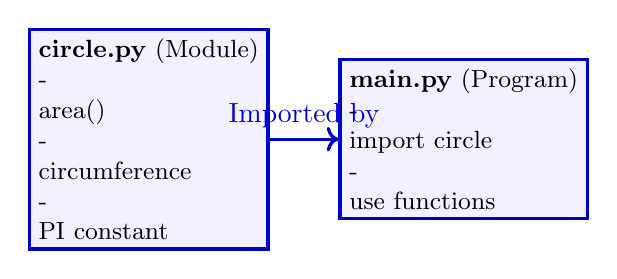
\begin{tikzpicture}[
            node distance=4cm,
            auto,
            block/.style={
                rectangle,
                draw=blue!80!black,
                fill=blue!5,
                very thick,
                minimum width=3cm,
                minimum height=2cm,
                align=left,
                font=\small
            }
        ]
            % Nodes
            \node[block] (circle) {\textbf{circle.py} (Module)\\-\\area()\\-\\circumference\\-\\PI constant};
            \node[block, right of=circle] (main) {\textbf{main.py} (Program)\\-\\import circle\\-\\use functions};

            % Arrow
            \draw[->, very thick, blue!80!black] (circle) -- node[above] {Imported by} (main);
        \end{tikzpicture}
    \end{center}

    \textbf{File 1: circle.py (Module)}
    \begin{lstlisting}[language=Python]
# circle.py - Circle calculation module
import math

# Constants
PI = math.pi

def area(radius):
    """Calculate area of circle"""
    if radius < 0:
        return "Radius cannot be negative"
    return PI * radius * radius

def circumference(radius):
    """Calculate circumference of circle"""
    if radius < 0:
        return "Radius cannot be negative"
    return 2 * PI * radius

def display_info():
    """Display module information"""
    print("Circle Module - Version 1.0")
    print("Functions: area(), circumference()")
    \end{lstlisting}

    \textbf{File 2: main.py (Main Program)}
    \begin{lstlisting}[language=Python]
# main.py - Main program using circle module
import circle

# Get radius from user
radius = float(input("Enter radius: "))

# Calculate using module functions
circle_area = circle.area(radius)
circle_circumference = circle.circumference(radius)

# Display results
print(f"Circle with radius {radius}:")
print(f"Area: {circle_area:.2f}")
print(f"Circumference: {circle_circumference:.2f}")

# Display module info
circle.display_info()
    \end{lstlisting}

    \begin{itemize}
        \item \textbf{Modular Design}: Organizes functions in a separate file
        \item \textbf{Reusability}: Module can be used in multiple programs
        \item \textbf{Namespace Management}: Functions are accessed via module prefix
    \end{itemize}
    \begin{mnemonicbox}Import Calculate Display\end{mnemonicbox}
\end{solutionbox}

\questionmarks{2(a) OR}{3}{Explain Nested Tuple with example.}
\begin{solutionbox}
    \textbf{Nested Tuple} contains other tuples inside it, creating a hierarchical data structure.

    \textbf{Nested Tuple Features:}
    \begin{center}
        \begin{tabulary}{\linewidth}{L L}
            \toprule
            \textbf{Feature} & \textbf{Description} \\
            \midrule
            \textbf{Multi-dimensional} & 2D or 3D data structure \\
            \textbf{Immutable} & Immutable at all levels \\
            \textbf{Indexing} & Access using multiple square brackets \\
            \textbf{Heterogeneous} & Can store different data types \\
            \bottomrule
        \end{tabulary}
    \end{center}

    \begin{lstlisting}[language=Python]
# Nested Tuple Example
student_records = (
    ("Raj", 20, ("IT", 2)),
    ("Priya", 19, ("CS", 1)), 
    ("Amit", 21, ("IT", 3))
)

# Accessing nested elements
print("First student:", student_records[0])
print("First student name:", student_records[0][0])
print("First student course:", student_records[0][2][0])

# Iterating through nested tuple
for student in student_records:
    name, age, (course, semester) = student
    print(f"{name} - Age: {age}, Course: {course}, Sem: {semester}")
    \end{lstlisting}

    \begin{itemize}
        \item \textbf{Data Organization}: Useful for grouping related data
        \item \textbf{Immutable Structure}: Structure cannot be changed once created
        \item \textbf{Efficient Access}: Fast index-based access
    \end{itemize}
    \begin{mnemonicbox}Nested = Tuple Inside Tuple\end{mnemonicbox}
\end{solutionbox}

\questionmarks{2(b) OR}{4}{What is PIP? Write the syntax to install and uninstall python packages.}
\begin{solutionbox}
    \textbf{PIP} (Pip Installs Packages) is a Python package installer that downloads and installs packages from PyPI.

    \textbf{PIP Commands:}
    \begin{center}
        \begin{tabulary}{\linewidth}{L L L}
            \toprule
            \textbf{Command} & \textbf{Syntax} & \textbf{Description} \\
            \midrule
            \textbf{Install} & \code{pip install package} & Installs package \\
            \textbf{Uninstall} & \code{pip uninstall package} & Removes package \\
            \textbf{List} & \code{pip list} & Shows installed packages \\
            \textbf{Show} & \code{pip show package} & Displays package info \\
            \textbf{Upgrade} & \code{pip install --upgrade pkg} & Updates package \\
            \bottomrule
        \end{tabulary}
    \end{center}

    \begin{lstlisting}[language=Python]
# PIP Command Examples (Run in Terminal/Command Prompt)

# Install a package
# pip install requests

# Install specific version
# pip install Django==3.2.0

# Uninstall a package  
# pip uninstall numpy

# List all installed packages
# pip list

# Show package information
# pip show matplotlib

# Upgrade a package
# pip install --upgrade pandas

# Install from requirements file
# pip install -r requirements.txt
    \end{lstlisting}

    \begin{itemize}
        \item \textbf{Package Management}: Can easily manage third-party libraries
        \item \textbf{Version Control}: Specific versions can be installed
        \item \textbf{Dependency Resolution}: Required dependencies are installed automatically
    \end{itemize}
    \begin{mnemonicbox}PIP = Package Install Python\end{mnemonicbox}
\end{solutionbox}

\questionmarks{2(c) OR}{7}{Explain different ways of importing package. How are modules and packages connected to each other?}
\begin{solutionbox}
    Different ways of imports in Python are important for code organization and namespace management.

    \textbf{Import Methods:}
    \begin{center}
        \begin{tabulary}{\linewidth}{L L L}
            \toprule
            \textbf{Method} & \textbf{Syntax} & \textbf{Usage} \\
            \midrule
            \textbf{Basic Import} & \code{import module} & Full module name required \\
            \textbf{From Import} & \code{from module import function} & Direct function access \\
            \textbf{Alias Import} & \code{import module as alias} & Short name for module \\
            \textbf{Star Import} & \code{from module import *} & Import all functions \\
            \textbf{Package Import} & \code{from package import module} & Import from package \\
            \bottomrule
        \end{tabulary}
    \end{center}

    \begin{lstlisting}[language=Python]
# Different Import Ways

# 1. Basic Import
import math
result = math.sqrt(16)

# 2. From Import
from math import sqrt, pi
result = sqrt(16)
area = pi * 5 * 5

# 3. Alias Import
import numpy as np
array = np.array([1, 2, 3])

# 4. Star Import (not recommended)
from math import *
result = cos(0)

# 5. Package Import
from mypackage import module1
from mypackage.subpackage import module3
    \end{lstlisting}

    \textbf{Module-Package Connection:}
    \begin{itemize}
        \item \textbf{Modules}: Single .py files containing Python code
        \item \textbf{Packages}: Directories containing multiple modules with \code{\_\_init\_\_.py}
        \item \textbf{Namespace}: Packages create hierarchical namespace structure
        \item \textbf{\_\_init\_\_.py}: Makes directory a package and controls imports
    \end{itemize}
    \begin{mnemonicbox}Import From As Star Package\end{mnemonicbox}
\end{solutionbox}

\section*{Question 3}

\questionmarks{3(a)}{3}{Describe Runtime Error and Syntax Error. Explain with example.}
\begin{solutionbox}
    \textbf{Error Types Comparison:}
    \begin{center}
        \begin{tabulary}{\linewidth}{L L L L}
            \toprule
            \textbf{Error Type} & \textbf{When Occurs} & \textbf{Detection} & \textbf{Example} \\
            \midrule
            \textbf{Syntax Error} & Code parsing time & Before execution & Missing colon \\
            \textbf{Runtime Error} & During execution & While running & Zero division \\
            \textbf{Logic Error} & Always & After execution & Wrong logic \\
            \bottomrule
        \end{tabulary}
    \end{center}

    \begin{lstlisting}[language=Python]
# Syntax Error Example
# print("Hello World"  # Missing closing parenthesis
# SyntaxError: unexpected EOF while parsing

# Runtime Error Examples
try:
    # ZeroDivisionError
    result = 10 / 0
except ZeroDivisionError:
    print("Cannot divide by zero")

try:
    # FileNotFoundError  
    file = open("nonexistent.txt", "r")
except FileNotFoundError:
    print("File not found")
    \end{lstlisting}

    \begin{itemize}
        \item \textbf{Syntax Errors}: Detected before code runs
        \item \textbf{Runtime Errors}: occur during program execution
        \item \textbf{Prevention}: Exception handling handles runtime errors
    \end{itemize}
    \begin{mnemonicbox}Syntax Before, Runtime During\end{mnemonicbox}
\end{solutionbox}

\questionmarks{3(b)}{4}{What is Exception handling in Python? Explain with example.}
\begin{solutionbox}
    \textbf{Exception handling} is a mechanism that gracefully handles runtime errors and prevents program crashes.

    \textbf{Exception Handling Keywords:}
    \begin{center}
        \begin{tabulary}{\linewidth}{L L L}
            \toprule
            \textbf{Keyword} & \textbf{Purpose} & \textbf{Description} \\
            \midrule
            \textbf{try} & Code prone to exception & Risk code block \\
            \textbf{except} & To handle exception & Error handling block \\
            \textbf{finally} & Always executed & Cleanup code \\
            \textbf{else} & If no exception & Success code block \\
            \textbf{raise} & To raise manual exception & Custom error throwing \\
            \bottomrule
        \end{tabulary}
    \end{center}

    \begin{lstlisting}[language=Python]
# Exception Handling Example
def safe_division(a, b):
    try:
        # Code that might raise exception
        result = a / b
        print(f"Division successful: {result}")
        
    except ZeroDivisionError:
        # Handle specific exception
        print("Error: Cannot divide by zero")
        result = None
        
    except TypeError:
        # Handle type errors
        print("Error: Invalid data types")
        result = None
        
    else:
        # Executes if no exception
        print("Division completed successfully")
        
    finally:
        # Always executes
        print("Division operation finished")
        
    return result

# Test the function
safe_division(10, 2)   # Normal case
safe_division(10, 0)   # Zero division
safe_division(10, "a") # Type error
    \end{lstlisting}

    \begin{itemize}
        \item \textbf{Error Prevention}: Prevents program from crashing
        \item \textbf{Graceful Handling}: Provides user-friendly error messages
        \item \textbf{Resource Management}: Cleanup operations in finally block
    \end{itemize}
    \begin{mnemonicbox}Try Except Finally Else Raise\end{mnemonicbox}
\end{solutionbox}

\questionmarks{3(c)}{7}{Create a function for division of two numbers, if the value of any argument is non-integer then raise the error or if second argument is 0 then raise the error.}
\begin{solutionbox}
    Creating custom exception handling function is important for validation and error control.

    \begin{lstlisting}[language=Python]
def safe_integer_division(num1, num2):
    """
    Divide two numbers with validation
    Raises TypeError if arguments are not integers
    Raises ZeroDivisionError if second argument is 0
    """
    
    # Check if both arguments are integers
    if not isinstance(num1, int):
        raise TypeError(f"First argument must be integer, got {type(num1).__name__}")
    
    if not isinstance(num2, int):
        raise TypeError(f"Second argument must be integer, got {type(num2).__name__}")
    
    # Check for zero division
    if num2 == 0:
        raise ZeroDivisionError("Cannot divide by zero")
    
    # Perform division
    result = num1 / num2
    return result

# Test the function with different cases
def test_division():
    test_cases = [
        (10, 2),      # Valid case
        (15, 3),      # Valid case  
        (10, 0),      # Zero division error
        (10.5, 2),    # Non-integer first argument
        (10, 2.5),    # Non-integer second argument
        ("10", 2),    # String argument
    ]
    
    for num1, num2 in test_cases:
        try:
            result = safe_integer_division(num1, num2)
            print(f"{num1} / {num2} = {result}")
            
        except TypeError as e:
            print(f"Type Error: {e}")
            
        except ZeroDivisionError as e:
            print(f"Zero Division Error: {e}")
            
        except Exception as e:
            print(f"Unexpected Error: {e}")
        
        print("-" * 40)

# Run tests
test_division()
    \end{lstlisting}

    \begin{itemize}
        \item \textbf{Input Validation}: Checks type and value of arguments
        \item \textbf{Custom Errors}: Raises specific exceptions
        \item \textbf{Error Messages}: Clear and descriptive error messages
    \end{itemize}
    \begin{mnemonicbox}Validate Type, Check Zero, Divide Safe\end{mnemonicbox}
\end{solutionbox}

\questionmarks{3(a) OR}{3}{Describe any five built-in exceptions in Python.}
\begin{solutionbox}
    \textbf{Built-in Exceptions:}
    \begin{center}
        \begin{tabulary}{\linewidth}{L L L}
            \toprule
            \textbf{Exception} & \textbf{Cause} & \textbf{Example} \\
            \midrule
            \textbf{ValueError} & Invalid value for operation & \code{int("abc")} \\
            \textbf{TypeError} & Wrong data type & \code{"5" + 5} \\
            \textbf{IndexError} & Index out of range & \code{list[10]} \\
            \textbf{KeyError} & Dictionary key not found & \code{dict["missing"]} \\
            \textbf{FileNotFoundError} & File does not exist & \code{open("missing.txt")} \\
            \bottomrule
        \end{tabulary}
    \end{center}

    \begin{itemize}
        \item \textbf{Automatic Detection}: Python automatically raises these exceptions
        \item \textbf{Specific Handling}: Each exception has a specific purpose
        \item \textbf{Inheritance}: All exceptions inherit from BaseException class
    \end{itemize}
    \begin{mnemonicbox}Value Type Index Key File\end{mnemonicbox}
\end{solutionbox}

\questionmarks{3(b) OR}{4}{Explain try...except...else...finally block with example.}
\begin{solutionbox}
    \textbf{Exception Block Structure:}
    \begin{center}
        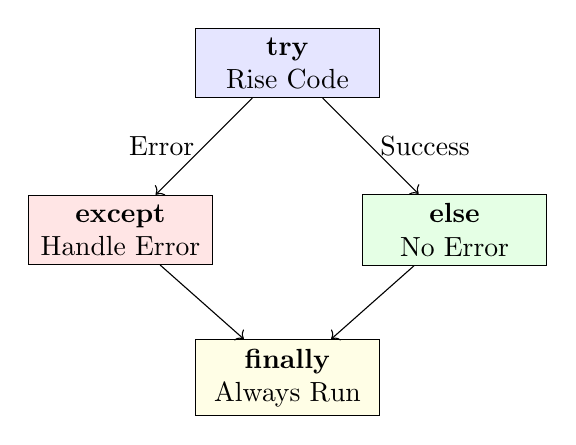
\begin{tikzpicture}[node distance=2cm, auto]
            \node (try) [rectangle, draw, fill=blue!10, text width=6em, text centered] {\textbf{try}\\Rise Code};
            \node (except) [rectangle, draw, fill=red!10, text width=6em, text centered, below left of=try, node distance=3cm] {\textbf{except}\\Handle Error};
            \node (else) [rectangle, draw, fill=green!10, text width=6em, text centered, below right of=try, node distance=3cm] {\textbf{else}\\No Error};
            \node (finally) [rectangle, draw, fill=yellow!10, text width=6em, text centered, below of=try, node distance=4cm] {\textbf{finally}\\Always Run};

            \draw [->] (try) -- node [left] {Error} (except);
            \draw [->] (try) -- node [right] {Success} (else);
            \draw [->] (except) -- (finally);
            \draw [->] (else) -- (finally);
        \end{tikzpicture}
    \end{center}

    \begin{lstlisting}[language=Python]
# Complete Exception Block Example
def file_operation(filename):
    try:
        # Try to open file
        f = open(filename, "r")
        print("File opened successfully")
        
    except FileNotFoundError:
        # Handle if file missing
        print("Error: File not found")
        
    else:
        # Run if no error occurred
        print("Reading file content...")
        print(f.read())
        f.close()
        
    finally:
        # Always runs
        print("File operation attempt finished")

# Test with existing and missing files
file_operation("existing.txt")
file_operation("missing.txt")
    \end{lstlisting}

    \begin{itemize}
        \item \textbf{Else Block}: Executes only if try block raises no exception
        \item \textbf{Finally Block}: Executes regardless of error (cleanup code)
        \item \textbf{Complete Flow}: Covers all possibilities of execution
    \end{itemize}
    \begin{mnemonicbox}Try Exception Else Finally\end{mnemonicbox}
\end{solutionbox}

\questionmarks{3(c) OR}{7}{Write a user defined exception that could be raised when the text entered by a user consists of less than 10 characters.}
\begin{solutionbox}
    User-defined exceptions allow custom validation logic.

    \begin{lstlisting}[language=Python]
class ShortTextError(Exception):
    """Custom exception for text validation"""
    def __init__(self, length):
        self.length = length
        self.message = f"Text too short ({length} chars). Minimum 10 required."
        super().__init__(self.message)

def validate_text():
    while True:
        try:
            # Get user input
            text = input("Enter text (min 10 chars): ")
            
            # Check length
            if len(text) < 10:
                raise ShortTextError(len(text))
            
            print(f"Valid text accepted: {text}")
            break
            
        except ShortTextError as e:
            print(f"Error: {e}")
            print("Please try again.\n")
            
        except Exception as e:
            print(f"Unexpected error: {e}")

# Run the validation
print("--- Text Validation Program ---")
# validate_text() # Uncomment to run
    \end{lstlisting}

    \begin{itemize}
        \item \textbf{Inheritance}: Custom exception class inherits from \code{Exception}
        \item \textbf{Raising}: \code{raise} keyword used to trigger exception
        \item \textbf{Usage}: Helps in implementing domain-specific constraints
    \end{itemize}
    \begin{mnemonicbox}Class Inherit Raise Catch\end{mnemonicbox}
\end{solutionbox}

\section*{Question 4}

\questionmarks{4(a)}{3}{Write five points on difference between Text File and Binary File.}
\begin{solutionbox}
    \textbf{Text vs Binary File:}
    \begin{center}
        \begin{tabulary}{\linewidth}{L L L}
            \toprule
            \textbf{Feature} & \textbf{Text File} & \textbf{Binary File} \\
            \midrule
            \textbf{Content} & Human readable characters & Machine readable (0s and 1s) \\
            \textbf{Encoding} & Uses encoding (ASCII/UTF-8) & No encoding used \\
            \textbf{Extensions} & .txt, .py, .csv & .bin, .jpg, .exe \\
            \textbf{EOL} & Handles Newline translation & No translation \\
            \textbf{Processing} & Slower processing & Faster processing \\
            \bottomrule
        \end{tabulary}
    \end{center}

    \begin{itemize}
        \item \textbf{Readability}: Text files can be opened in simple editors
        \item \textbf{Portability}: Binary files are continuous stream of bytes
        \item \textbf{Usage}: Text for documents, Binary for images/videos/data
    \end{itemize}
    \begin{mnemonicbox}Text Human, Binary Machine\end{mnemonicbox}
\end{solutionbox}

\questionmarks{4(b)}{4}{Write a program to read the data from a file and separate the uppercase character and lowercase character into two separate files.}
\begin{solutionbox}
    File processing involves reading, analyzing, and writing to multiple files.

    \begin{lstlisting}[language=Python]
def separate_case_chars(source_file):
    try:
        # Strings to store separated characters
        upper_chars = ""
        lower_chars = ""
        
        # Read source file
        with open(source_file, "r") as f:
            content = f.read()
            
            # Process each character
            for char in content:
                if char.isupper():
                    upper_chars += char
                elif char.islower():
                    lower_chars += char
        
        # Write uppercase characters
        with open("uppercase.txt", "w") as f:
            f.write(upper_chars)
            
        # Write lowercase characters
        with open("lowercase.txt", "w") as f:
            f.write(lower_chars)
            
        print("Characters separated successfully!")
        
    except FileNotFoundError:
        print("Source file not found")

# Create a sample file first
with open("input.txt", "w") as f:
    f.write("Hello World! Python Programming.")

# Run separation
separate_case_chars("input.txt")
    \end{lstlisting}

    \begin{itemize}
        \item \textbf{String Methods}: \code{isupper()} and \code{islower()} check case
        \item \textbf{File Handling}: Uses \code{with} statement for safe file operations
        \item \textbf{Data Separation}: Content is filtered into different streams
    \end{itemize}
    \begin{mnemonicbox}Read Loop Check Write\end{mnemonicbox}
\end{solutionbox}

\questionmarks{4(c)}{7}{Describe dump() and load() method. Explain with example.}
\begin{solutionbox}
    \code{dump()} and \code{load()} are part of \textbf{pickle} module used for object serialization.

    \textbf{Pickle Methods:}
    \begin{center}
        \begin{tabulary}{\linewidth}{L L L}
            \toprule
            \textbf{Method} & \textbf{Purpose} & \textbf{Mode} \\
            \midrule
            \textbf{dump(obj, file)} & Serializes object to file & Write Binary ('wb') \\
            \textbf{load(file)} & Deserializes object from file & Read Binary ('rb') \\
            \bottomrule
        \end{tabulary}
    \end{center}

    \begin{lstlisting}[language=Python]
import pickle

# Data to serialize
student = {
    "name": "Rahul",
    "roll": 101,
    "marks": [85, 90, 88]
}

# DUMP Example
try:
    with open("data.pkl", "wb") as f:
        pickle.dump(student, f)
    print("Data dumped successfully")
except Exception as e:
    print(f"Error: {e}")

# LOAD Example
try:
    with open("data.pkl", "rb") as f:
        loaded_data = pickle.load(f)
    print("Data loaded successfully:")
    print(loaded_data)
except Exception as e:
    print(f"Error: {e}")
    \end{lstlisting}

    \begin{itemize}
        \item \textbf{Serialization}: Converting object to byte stream (Pickling)
        \item \textbf{Deserialization}: Converting byte stream back to object (Unpickling)
        \item \textbf{Persistence}: Allows saving state of objects to disk
    \end{itemize}
    \begin{mnemonicbox}Dump Store, Load Restore\end{mnemonicbox}
\end{solutionbox}

\questionmarks{4(a) OR}{3}{List different types of file modes provided by python for file operations and explain their uses.}
\begin{solutionbox}
    \textbf{Python File Modes:}
    \begin{center}
        \begin{tabulary}{\linewidth}{L L L}
            \toprule
            \textbf{Mode} & \textbf{Name} & \textbf{Description} \\
            \midrule
            \textbf{'r'} & Read & Default mode. Opens for reading. \\
            \textbf{'w'} & Write & Opens for writing. Overwrites file. \\
            \textbf{'a'} & Append & Opens for writing. Appends to end. \\
            \textbf{'x'} & Create & Creates new file. Fails if exists. \\
            \textbf{'b'} & Binary & Binary mode (e.g., 'rb', 'wb'). \\
            \textbf{'+'} & Update & Read and Write (e.g., 'r+', 'w+'). \\
            \bottomrule
        \end{tabulary}
    \end{center}

    \begin{itemize}
        \item \textbf{Safety}: 'x' prevents accidental overwriting
        \item \textbf{Binary}: 'b' must be used for non-text files
        \item \textbf{Combination}: '+ can be combined with other modes
    \end{itemize}
    \begin{mnemonicbox}Read Write Append Create\end{mnemonicbox}
\end{solutionbox}

\questionmarks{4(b) OR}{4}{Describe readline() and writeline() functions of the file.}
\begin{solutionbox}
    \textbf{Note}: Python has \code{writelines()} but no \code{writeline()}.

    \textbf{Line Operations:}
    \begin{center}
        \begin{tabulary}{\linewidth}{L L L}
            \toprule
            \textbf{Function} & \textbf{Purpose} & \textbf{Example} \\
            \midrule
            \textbf{readline()} & Reads single line & \code{line = f.readline()} \\
            \textbf{readlines()} & Reads all lines into list & \code{lines = f.readlines()} \\
            \textbf{writelines()} & Writes list of strings & \code{f.writelines(list)} \\
            \bottomrule
        \end{tabulary}
    \end{center}

    \begin{lstlisting}[language=Python]
# Write lines
lines = ["First Line\n", "Second Line\n"]
with open("demo.txt", "w") as f:
    f.writelines(lines)

# Read lines
with open("demo.txt", "r") as f:
    line1 = f.readline()
    print(f"Read 1: {line1.strip()}")
    
    line2 = f.readline()
    print(f"Read 2: {line2.strip()}")
    \end{lstlisting}

    \begin{itemize}
        \item \textbf{Sequential}: readline moves pointer line by line
        \item \textbf{List Support}: writelines accepts iterable (list/tuple)
        \item \textbf{Memory}: readline is efficient for large files
    \end{itemize}
    \begin{mnemonicbox}Read One, Write Many\end{mnemonicbox}
\end{solutionbox}

\questionmarks{4(c) OR}{7}{Write a python program to demonstrate seek() and tell() methods.}
\begin{solutionbox}
    \code{seek()} moves file pointer, \code{tell()} returns current position.

    \begin{lstlisting}[language=Python]
# Seek and Tell Demonstration
filename = "seek_demo.txt"

# Create file
with open(filename, "w") as f:
    f.write("Hello Python World")

# Read operations
with open(filename, "r") as f:
    # Initial position
    print(f"Start Position: {f.tell()}")  # 0
    
    # Read first 5 chars
    print(f"Read: {f.read(5)}")          # Hello
    print(f"Current Position: {f.tell()}") # 5
    
    # Seek to start
    f.seek(0)
    print(f"After seek(0): {f.tell()}")   # 0
    
    # Seek to specific position
    f.seek(6)
    print(f"After seek(6): {f.read(6)}")  # Python
    
    # Seek from end (requires binary mode usually, or specific syntax)
    # f.seek(0, 2) moves to end
    \end{lstlisting}

    \begin{center}
        \begin{tabulary}{\linewidth}{L L}
            \toprule
            \textbf{Method} & \textbf{Syntax} \\
            \midrule
            \textbf{tell()} & \code{pos = f.tell()} \\
            \textbf{seek()} & \code{f.seek(offset, whence)} \\
            \bottomrule
        \end{tabulary}
    \end{center}

    \begin{itemize}
        \item \textbf{Navigation}: Allows random access in files
        \item \textbf{Whence}: 0=Start, 1=Current, 2=End
        \item \textbf{Binary}: Relative seeking works best in binary mode
    \end{itemize}
    \begin{mnemonicbox}Tell Position, Seek Location\end{mnemonicbox}
\end{solutionbox}

\section*{Question 5}

\questionmarks{5(a)}{3}{Draw the shape of circle and rectangle using turtle and fill with red color.}
\begin{solutionbox}
    \begin{lstlisting}[language=Python]
import turtle

t = turtle.Turtle()

# Fill color set to red
t.fillcolor("red")

# Draw Circle
t.begin_fill()
t.circle(50)      # Draw circle with radius 50
t.end_fill()

# Move to new position
t.penup()
t.goto(100, 0)
t.pendown()

# Draw Rectangle
t.begin_fill()
for _ in range(2):
    t.forward(100) # Length
    t.right(90)
    t.forward(50)  # Width
    t.right(90)
t.end_fill()

turtle.done()
    \end{lstlisting}

    \begin{itemize}
        \item \textbf{begin\_fill()}: Starts filling shape
        \item \textbf{end\_fill()}: Completes filling shape
        \item \textbf{Geometry}: Circle and loop-based rectangle drawing
    \end{itemize}
    \begin{mnemonicbox}Begin Fill End\end{mnemonicbox}
\end{solutionbox}

\questionmarks{5(b)}{4}{Explain various inbuilt methods for changing the direction of turtle.}
\begin{solutionbox}
    \textbf{Turtle Direction Methods:}
    \begin{center}
        \begin{tabulary}{\linewidth}{L L L}
            \toprule
            \textbf{Method} & \textbf{Description} & \textbf{Example} \\
            \midrule
            \textbf{right(angle)} & Turn right by angle & \code{t.right(90)} \\
            \textbf{left(angle)} & Turn left by angle & \code{t.left(45)} \\
            \textbf{setheading(angle)} & Set absolute angle & \code{t.setheading(0)} \\
            \textbf{towards(x,y)} & Point towards coords & \code{t.towards(0,0)} \\
            \bottomrule
        \end{tabulary}
    \end{center}

    \begin{lstlisting}[language=Python]
# Direction Examples
import turtle
t = turtle.Turtle()

t.forward(100)
t.right(90)       # Turn 90 degrees right
t.forward(50)
t.left(45)        # Turn 45 degrees left
t.setheading(180) # Face West (180 degrees)
    \end{lstlisting}

    \begin{itemize}
        \item \textbf{Relative}: right/left are relative to current direction
        \item \textbf{Absolute}: setheading uses 0-360 degree system
        \item \textbf{Navigation}: Essential for drawing complex shapes
    \end{itemize}
    \begin{mnemonicbox}Right Left Heading Towards\end{mnemonicbox}
\end{solutionbox}

\questionmarks{5(c)}{7}{Write a python program to draw rainbow using turtle.}
\begin{solutionbox}
    Rainbow drawing utilizes concentric semi-circles with VIBGYOR colors.

    \begin{lstlisting}[language=Python]
import turtle

def draw_rainbow():
    # Setup screen
    wn = turtle.Screen()
    wn.bgcolor("skyblue")
    
    # Setup turtle
    t = turtle.Turtle()
    t.speed(5)
    t.pensize(10)
    
    # Rainbow colors (VIBGYOR reversed)
    colors = ['violet', 'indigo', 'blue', 'green', 
              'yellow', 'orange', 'red']
    
    # Initial position parameters
    radius = 180
    
    # Draw arcs
    for color in colors:
        t.penup()
        t.goto(0, -50)     # Center bottom
        t.setheading(90)   # Face up
        t.right(90)        # Face right (0 deg)
        t.forward(radius)  # Move to start of arc
        t.left(90)         # Face up again
        t.pendown()
        
        t.pencolor(color)
        t.circle(radius, 180) # Draw semi-circle
        
        radius -= 20      # Decrease radius for next color
    
    t.hideturtle()
    turtle.done()

draw_rainbow()
    \end{lstlisting}

    \begin{itemize}
        \item \textbf{Looping}: Iterates through list of colors
        \item \textbf{Concentric}: Radius decreases for each inner arc
        \item \textbf{Arc}: \code{circle(radius, 180)} draws half circle
    \end{itemize}
    \begin{mnemonicbox}Colors Loop Radius Circle\end{mnemonicbox}
\end{solutionbox}

\end{document}
